\chapter{Architettura software}
\label{cap:architetturasw}

Per semplificare l'implementazione e agevolare il riuso del codice esistente, il software è stato realizzato utilizzando ROS (Robot Operating System) \cite{rosweb}. Si tratta di un middleware pensato per applicazioni robotiche costituite da un elevato numero di moduli, relativamente indipendenti, che interagiscono tra loro.

Un sistema realizzato con ROS è suddiviso in un certo numero di \emph{nodi}, ovvero semplici processi\footnote{attualmente ROS supporta C++ e Python} indipendenti, che vengono eseguiti in parallelo e svolgono ciascuno una funzione elementare. Per migliorare l'organizzazione (e la distribuzione) del codice sorgente, i nodi possono poi essere raggruppati in \emph{package}. A loro volta, un gruppo di package può formare uno \emph{stack}. ROS mette a disposizione due differenti tecniche con cui i nodi possono comunicare tra loro:
\begin{itemize}
 \item un paradigma ``publish-subscribe'': i nodi pubblicano (\emph{publish}) messaggi su un certo argomento (\emph{topic}). I destinatari della comunicazione sono i nodi iscritti (\emph{subscribe}) a quel topic.
 \item l'invocazione di \emph{servizi} esposti da altri nodi, con la possibilità di ricevere una risposta, secondo una semantica simile a quella di una chiamata di procedura remota (RPC)
\end{itemize}

Oltre a funzionare come middleware di comunicazione interprocesso, ROS mette a disposizione alcuni programmi grafici e testuali, e funzioni di libreria che forniscono funzioni utili allo sviluppo di applicazioni robotiche.

Il sistema da noi realizzato risulta quindi composto da vari nodi. Ciascuno di essi è contenuto in un package omonimo all'interno della directory principale del progetto. In figura \ref{fig:schemanodi} è rappresentata l'architettura generale del sistema: in particolare i vari nodi e le dipendenze dalle librerie esterne a ROS. Le frecce rappresentano la comunicazione tra nodi (messaggi scambiati e servizi invocati) e i canali di comunicazione tra il software presente sull'unità di elaborazione e il robot.

\begin{figure}[h]
\resizebox{\linewidth}{!}{%
\begin{tikzpicture}[node distance=1cm, auto]
\tikzset{
   mynode/.style={rectangle,rounded corners,draw=black, top color=white, bottom color=white!50, thick, inner sep=1em, minimum size=3em, text centered},
   mynode2/.style={rectangle,rounded corners,draw=black, top color=white, bottom color=white!50, dashed, inner sep=1em, minimum size=1em, text centered},
}  
\node[mynode] (spykee) {\textbf{SpyKee}}; 
\node[mynode, below=4cm of spykee] (echoes) {\textbf{Echoes}}; 
\node[mynode, right=5cm of spykee] (vision) {\textbf{Vision}}; 
\node[mynode, below right=3cm of vision] (isaac) {\textbf{IsAac}}; 
\node[mynode2, below=1cm of isaac] (brian) {\emph{Mr. BRIAN}}; 
\node[mynode2, below left= 2cm of spykee] (robot) {\emph{Robot}}; 
\node[mynode2, above=1cm of vision] (opencv) {\emph{OpenCV + Blob Growing Algorithm}}; 
 
\draw[->, >=latex', shorten >=2pt, shorten <=2pt, bend left=10, thick] 
     (spykee.east) to node[auto, swap] {\ttfamily{spykee\_camera}}(vision.west); 

\draw[->, >=latex', shorten >=2pt, shorten <=2pt, bend left=10, thick] 
     (isaac.west) to node[auto, swap] {\ttfamily{spykee\_motion}}(spykee.south); 

\draw[->, >=latex', shorten >=2pt, shorten <=2pt, bend right=20, thick] 
     (echoes.east) to node[auto,swap] {\ttfamily{\begin{tabular}{c}
	 sonar\_data \\
     rfid\_data \\
     towers\_data
  \end{tabular}
}}(isaac.west); 
     
\draw[->, >=latex', shorten >=2pt, shorten <=2pt, bend right=10, thick, dashed] 
     (isaac.west) to node[auto, swap] {{\ttfamily{led\_data}} (servizio)}(echoes.east); 

\draw[->, >=latex', shorten >=2pt, shorten <=2pt, bend left=30, thick] 
     (vision.east) to node[auto, swap] {{\ttfamily{vision\_results}}}(isaac.north); 

\draw[<->, >=latex', shorten >=2pt, shorten <=2pt, bend left=0, thin, dashed] 
     (isaac.south) to node[auto, swap] {}(brian.north); 

\draw[<->, >=latex', shorten >=2pt, shorten <=2pt, bend left=0, thin, dashed] 
     (vision.north) to node[auto, swap] {}(opencv.south); 

\draw[<->, >=latex', shorten >=2pt, shorten <=2pt, bend left=7, thin, dashed] 
     (robot.north) to node[auto, swap] {Wi-fi}(spykee.west); 

\draw[<->, >=latex', shorten >=2pt, shorten <=2pt, bend right=7, thin, dashed] 
     (robot.south) to node[auto, swap] {Zigbee}(echoes.west); 

% The swap command corrects the placement of the text.

\end{tikzpicture} 
} 
\medskip

\caption{Struttura generale del sistema} 
\label{fig:schemanodi}
\end{figure}

\section{SpyKee}
\emph{SpyKee} si occupa di interfacciare l'unità di elaborazione con le funzioni del robot che comunicano via Wi-Fi: permette di fornire i comandi ai cingoli e di ricevere le immagini catturate dalla telecamera. Questo nodo è frutto dell'adattamento a ROS di una libreria realizzata nei precedenti progetti, e ottenuta analizzando con un software di cattura dei pacchetti di rete la comunicazione tra il robot e il software di controllo per Microsoft Windows fornito dalla Meccano.

SpyKee pubblica messaggi di tipo \verb|std_msgs::CompressedImage| sull'argomento \verb|spykee_camera|, che contengono le immagini ricevute dalla telecamera compresse in formato JPEG. Inoltre sottoscrive messaggi di tipo \verb|SpyKee::Motion| sull'argomento \verb|spykee_motion|, contenenti i comandi da inviare ai cingoli. Tali comandi sono costituiti da due interi compresi tra $-90$ e $90$, che rappresentano la velocità tangenziale e angolare del robot, e vengono convertiti dal nodo nei corrispondenti comandi al cingolo destro e sinistro.

\section{Echoes}
\emph{Echoes} comunica via Zigbee con l'hardware aggiunto a posteriori al robot: sonar, led, lettore RFID, e ricevitori dei comandi inviati dagli interruttori posti sulle torri e sulle fabbriche.

Il nodo riceve i dati dalla porta seriale\footnote{di default viene utilizzato il device \texttt{/dev/ttyUSB0}, altrimenti il percorso deve essere fornito da riga di comando come primo argomento}, analizza le stringhe ricevute, e pubblica i messaggi contenenti i dati rilevati:
\begin{itemize}
	\item i messaggi di tipo \verb|Echoes::Sonar| sull'argomento \verb|sonar_data| contengono i dati ricevuti dai sonar (valori delle distanze dei quattro sonar montati sul robot, espresse in millimetri).
	\item i messaggi di tipo \verb|Echoes::Rfid| sull'argomento \verb|rfid_data| contengono semplicemente una stringa identificativa del tag RFID rilevato
	\item i messaggi di tipo \verb|Echoes::Tower| sull'argomento \verb|towers_data| contengono un intero che corrisponde all'id della torre (o della fabbrica) abbattuta
\end{itemize}
Inoltre, il nodo espone alcuni servizi che permettono di comandare i led presenti sul robot (\verb|green_led|, \verb|yellow_led| e \verb|red_led|), e un ulteriore servizio che consente di spegnere tutti i led (\verb|reset_led|). I led possono essere impostati nello stato di acceso, spento o lampeggiante. In particolare, per i led gialli e i led rossi, lo stato lampeggiante viene definito a livello dell'intero gruppo di led.

A causa dell'alto rumore presente nei valori provenienti dai sonar, il valore $x_k$ che viene pubblicato sul topic \verb|sonar_data| è filtrato attraverso un filtro a media mobile esponenziale. Questo significa che il dato pubblicato all'arrivo del $k$-esimo campione $x_{cur}$ registrato dal sonar è dato da
  \[ x_k = \alpha x_{cur} + (1 - \alpha) x_{k-1} \]
dove $\alpha = 0.3$, valore sufficientemente basso da ridurre il rumore ad alta frequenza presente nel segnale, ma comunque abbastanza alto da rendere l'aggiornamento dei valori reattivo, e riuscire ad evitare efficacemente gli ostacoli.

\section{Vision: identificazione degli oggetti}

\emph{Vision} si occupa di analizzare le immagini provenienti dalla telecamera di Spykee, per rilevare la presenza di una torre o di una fabbrica. 

Il nodo riceve da \emph{SpyKee} i messaggi contenenti le immagini e, analizzata l'immagine, pubblica un messaggio di tipo \verb|Vision::Results| sull'argomento \verb|vision_results|. Questo messaggio contiene i dati riguardanti gli oggetti trovati: la posizione rispetto al centro dell'immagine, una stima della distanza in centimetri, e l'altezza e la larghezza del blob in pixel.

Il cuore del nodo è un algoritmo, già utilizzato nel progetto \cite{docmandelli}, che si occupa di identificare all'interno dell'immagine dei blob sufficientemente uniformi e di colore ``simile'' a quello degli oggetti che si stanno cercando. L'analisi viene effettuata basandosi su un algoritmo di tipo KNN, che necessita di una prima fase di addestramento. Al termine di questa fase, viene generato un classificatore (contenuto in un file \verb|.kcc|), tramite il quale l'algoritmo è in grado di associare ad ogni pixel dell'immagine una classe di identificazione. Le classi riguardano i pixel di colore simile a quello di una torre (classe \verb|R|), oppure di una fabbrica (classe \verb|G|). Una volta effettuata la classificazione dei pixel dell'immagine, l'algoritmo per rileva all'interno dell'immagine i blob di interesse, e quindi stabilisce se è presente una torre o una fabbrica.

Il classificatore viene generato a partire da un file che contiene semplicemente un elenco di valori \verb|BGR| di pixel che si considerano del colore cercato. Per generare questo file è possibile utilizzare il nodo \emph{LittleEndian}: questo nodo carica le immagini da file oppure le riceve direttamente da \emph{SpyKee}, e consente di evidenziare nell'immagine le aree che corrispondono agli oggetti cercati. Alla fine, LittleEndian genera un file \verb|.dts| che contiene l'insieme dei valori. Per generare il classificatore, è sufficiente lanciare una volta \emph{Vision} indicando come parametro \verb|-L <filename.dts>|.

%TODO filtraggio etc?

\begin{nota}
È necessario prestare particolare attenzione nel training del classificatore, in quanto è una fase critica per il corretto funzionamento del gioco e il corretto riconoscimento degli oggetti.
\end{nota}

\section{RoboTower\_Game: la logica di gioco}
\begin{figure}
\centering
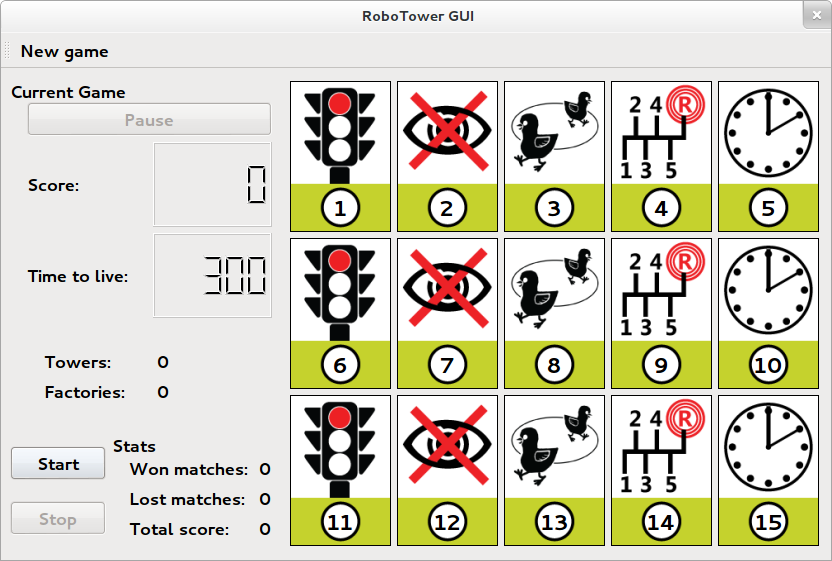
\includegraphics[scale=0.43]{images/rtgame}
\caption{Schermata principale dell'interfaccia di controllo del gioco}
\end{figure}

\emph{RoboTower\_Game} gestisce la logica ad ``alto livello'' del gioco e la comunicazione con l'utente tramite un'apposita interfaccia grafica, realizzata con le librerie Qt \cite{qtweb}. Si occupa di avviare e arrestare le partite, gestire lo stato del gioco, contare i punti, e tenere alcune semplici statistiche. Il nodo interagisce con gli altri processi:
\begin{itemize}
\item avviando e fermando il comportamento di basso livello del robot, a seconda dello stato corrente del gioco (pubblicando messaggi di tipo \verb|std_msgs::Bool| sull'argomento \verb|isaac_enable|)
\item ricevendo da \verb|Echoes| gli ID dei tag RFID letti e le informazioni riguardanti eventuali abbattimenti di torri o fabbriche
\item pubblicando messaggi di tipo \verb|std_msgs::String| relativi alle azioni speciali che devono essere eseguite dal robot (topic \verb|rfid_actions|), come spiegato nel seguito
\item invocando i servizi relativi all'accensione e allo spegnimento dei led relativi al punteggio
\end{itemize}

\begin{figure}[h]
{
\lstset{
  language=XML,
  morekeywords={encoding, robotower, config, time, points, goals, recharge, rfid, action, tag}}
\begin{lstlisting}
<robotower>
	<config>
		<time timetolive="300" setuptime="30" />
		<points tower="100" factory="30" />
		<goals towerid="4" factories="3" />
		<recharge tower="3" factory="2"/>
	</config>

	<rfid>
		<action name="lock_all">
			<tag id="4400F56CD1" num="1" />
			<tag id="4400F59195" num="2" />
			<tag id="4400F58B6D" num="3" />
		</action>
      
		<action name="disable_vision">
			<tag id="4400BDB1D9" num="4" />
			<tag id="4400BDC253" num="5" />
			<tag id="4B00DA3279" num="6" />
		</action>
	</rfid>
</robotower>
\end{lstlisting}
}
\caption{Il file di configurazione}
\label{fig:configfile}
\end{figure}

La maggior parte delle impostazioni di RoboTower\_Game possono essere configurate modificando il file \verb|robotower.xml|, che si trova nella directory \verb|RoboTower_Game|. Un esempio di file di configurazione corretto è riportato in figura \ref{fig:configfile}\footnote{per semplicità sono stati omessi alcuni tag RFID e le relative azioni}. Nel file è possibile specificare:
\begin{itemize}
\item I tempi del gioco (tag \lstinline|<time>|): l'attributo \lstinline|timetolive| permette di modificare la durata massima di un round del gioco, mentre l'attributo \lstinline|setuptime| controlla il tempo che deve trascorrere dall'inizio della partita (pressione del pulsante ``start'') e l'inizio del movimento del robot
\item I parametri con cui viene calcolato il punteggio (tag \lstinline|<points>|): durante la partita, ogni secondo viene aggiunto un certo numero di punti per ogni torre e fabbrica che non sono stati ancora distrutti, definiti dagli attributi \lstinline|tower| e \lstinline|factory|
\item I parametri relativi a torre e fabbriche (tag \lstinline|<goals>|): in particolare, il numero di fabbriche (\lstinline|factories|) e l'id dell'obiettivo che dev'essere considerato come torre (\lstinline|towerid|)
\item I parametri relativi al tempo di ricarica delle trappole (tag \lstinline|<recharge>|). Le trappole vengono completamente ricaricate dopo
\[\frac{100}{\texttt{tower} + \texttt{factories} \cdot \textrm{fabbriche attive}}\]
secondi da quando vengono attivate.
\end{itemize}
Il nodo si occupa inoltre di gestire i comportamenti ``speciali'' del robot, collegati alle trappole (tag RFID). Per ogni trappola, è necessario specificare, all'interno del blocco \lstinline|<action>| relativo all'azione associata, l'id e un numero (univoco) che viene utilizzato per identificarlo nell'interfaccia grafica. Le azioni che possono essere specificate (parametri \lstinline|name|) sono:
\begin{itemize}
\item \lstinline|lock_all|: blocca per 5 secondi i motori del robot
\item \lstinline|force_rotate|: costringe per 5 secondi il robot a ruotare su se stesso, inibendo i comandi diretti a uno dei due cingoli
\item \lstinline|disable_vision|: disabilita la visione del robot per 5 secondi
\item \lstinline|go_back|: blocca per 5 secondi l'avanzamento del robot, costringendolo a tornare indietro
\item \lstinline|modify_time|: modifica casualmente il tempo rimanente alla fine del round (sia in positivo che in negativo)
\end{itemize}
Una volta che viene letto un tag, questo viene disabilitato. I tag vengono ricaricati, uno alla volta, dopo un periodo di tempo che dipende dai parametri di configurazione impostati.

\section{IsAac: il comportamento del robot}
\emph{IsAac} si occupa di controllare il comportamento di ``basso livello'' del robot durante il gioco. In base ai dati provenienti dai sensori, gestisce il comportamento del robot, impostando i set-point per i cingoli e controllando l'accensione di alcuni led.

Il nodo riceve i messaggi pubblicati da \emph{Echoes} e \emph{Vision}, e invia comandi a \emph{SpyKee} (messaggi \verb|Spykee::Motion| sull'argomento \verb|spykee_motion|) riguardanti il controllo dei cingoli. Inoltre invoca il servizio \verb|led_data| esposto da Echoes per il controllo dei led gialli e del led verde posti sul robot. I led gialli lampeggiano quando \emph{IsAac} è attivo, sono spenti quando non è attivo, e rimangono accesi quando il robot è bloccato in una trappola. Il led verde lampeggia quando viene rilevata una torre o una fabbrica, altrimenti è spento.

\emph{IsAac} riceve da \emph{RoboTower\_Game} i comandi di attivazione e disattivazione, e le informazioni riguardanti il blocco del robot in una trappola (quando l'azione a cui è associata richiede la modifica dei dati provenienti dai sensori oppure dei comandi diretti agli attuatori, in caso contrario l'azione è implementata direttamente in \emph{RoboTower\_Game}).

Per l'implementazione di questo nodo, è stata sfruttata la libreria Mr. Brian, sviluppata dal Politecnico di Milano nel contesto di di MRT (Modular Robotic Toolkit) \cite{mrt}. Questa libreria consente di definire il comportamento da applicare al robot come un insieme di regole scritte in \emph{logica fuzzy}, utilizzando anche predicati che risultano dalla fuzzyficazione degli ingressi. La configurazione di Brian è basata su un insieme di file di testo: in questo modo è possibile modificare totalmente i comportamenti senza bisogno di ricompilare il codice sorgente. I file di configurazione, presenti nella cartella \verb|IsAac/config|, sono:
\begin{itemize}
\item \verb|behaviour.txt| contiene l'elenco, suddiviso per livelli, dei comportamenti (regole) che sono stati definiti. Ogni comportamento, costituito da un insieme di regole fuzzy, è contenuto in un file \verb|.rul|
\item \verb|ctof.txt| associa ad ogni dato crisp in ingresso un'insieme fuzzy, che verrà utilizzato per la fase di fuzzyficazione. Gli insiemi fuzzy sono definiti nel file \verb|shape_ctof.txt|.
\item \verb|s_ftoc.txt| definisce i valori in uscita da Brian, associandoli agli insiemi fuzzy da utilizzare per la defuzzyficazione. Gli insiemi sono definiti nel file \verb|s_shape.txt|
\item \verb|Predicate.ini| definisce i predicati fuzzy sulla base di variabili fuzzy e/o di altri predicati
\item \verb|Cando.ini| definisce le condizioni di attivazione per un determinato comportamento (le condizioni necessarie per cui eseguire quel comportamento sia sensato)
\item \verb|Want.ini| definisce le condizioni per cui è opportuno attivare un determinato comportamento
\end{itemize}
La suddivisione in livelli nel file \verb|behaviour.txt| permette di utilizzare come ingresso dati in uscita dai livelli precedenti, ed eventualmente cancellare anche le uscite impostate dai livelli precedenti. Nelle regole, infatti, è possibile utilizzare anche i predicati, definiti nel file \verb|PredicateActions.ini|, in cui è possibile far riferimento ai dati in uscita dai livelli precedenti a quello corrente utilizzando etichette della forma
\begin{center}\verb|Proposed<nome del dato in uscita>|\end{center}
dopo averle associate ad opportuni insiemi fuzzy nel file \verb|ctof.txt|. La suddivisione in livelli permette di rendere maggiormente modulari le regole fuzzy. All'interno del manuale di MRT \cite{mrtmanual} è presente la descrizione completa del funzionamento di Mr. Brian e della sintassi dei file di configurazione.

\begin{figure}[h]
\centering
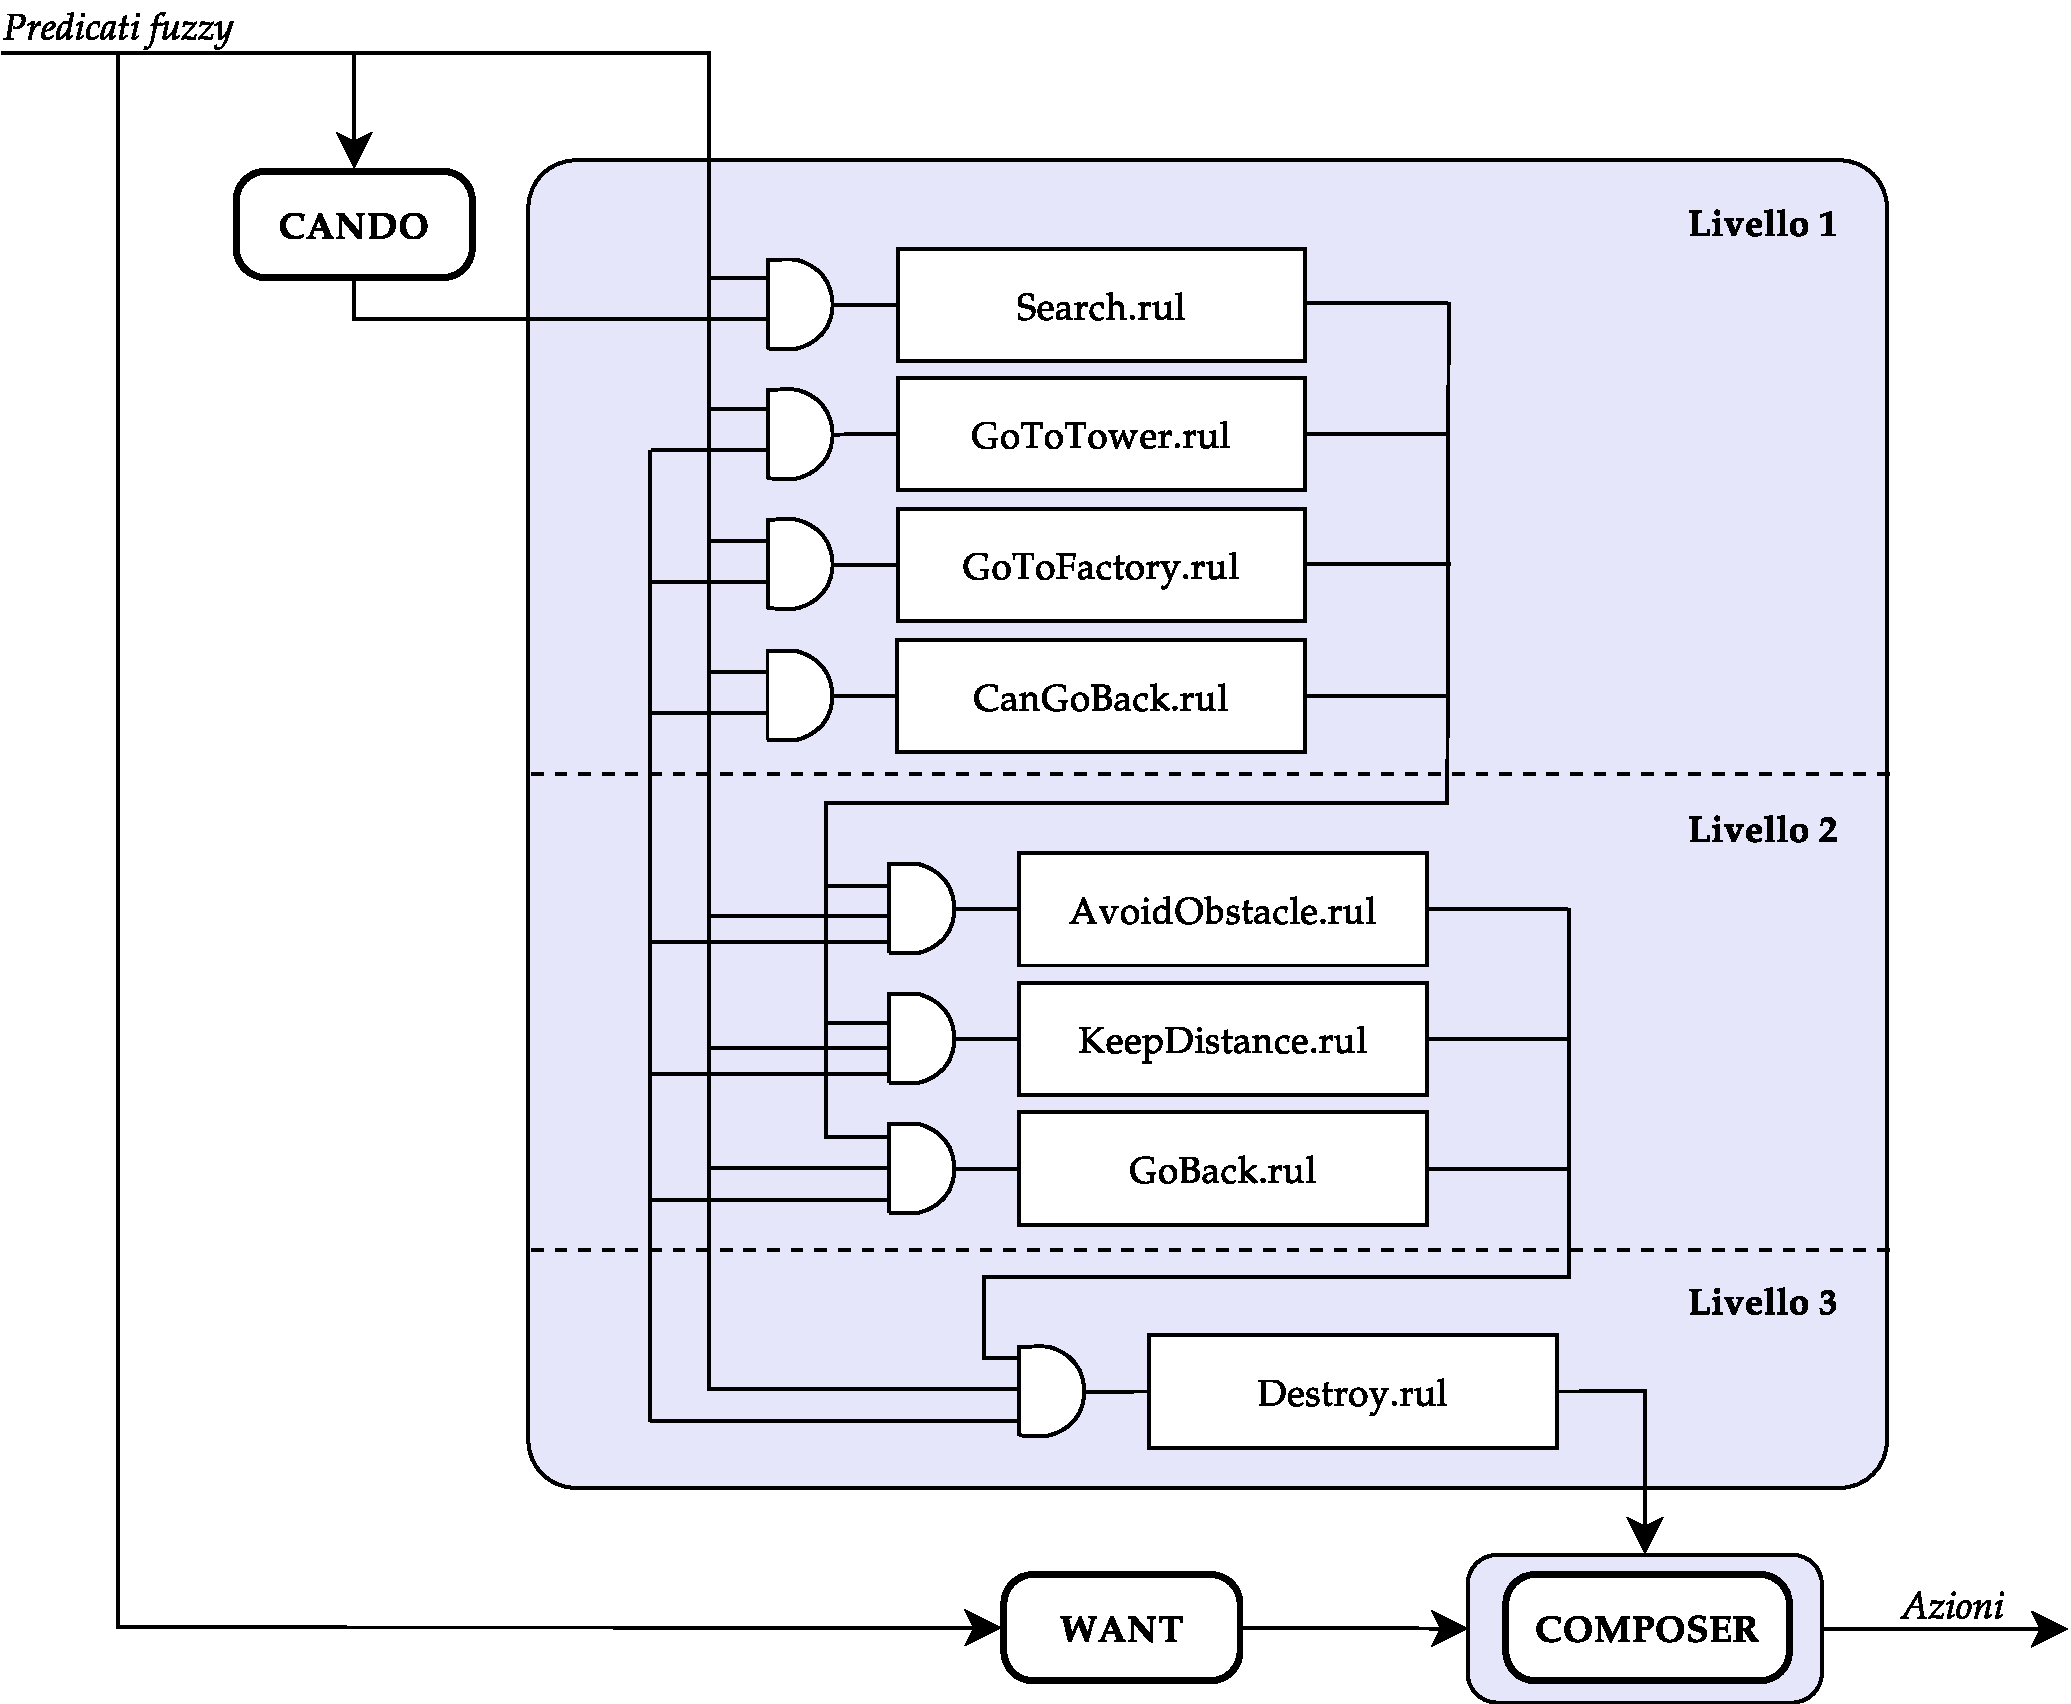
\includegraphics[scale=0.35]{images/schemafuzzy}
\caption{I comportamenti utilizzati da IsAac}
\label{fig:schemafuzzy}
\end{figure}

I comportamenti che sono stati implementati permettono al robot di:
\begin{itemize}
 \item Cercare casualmente la torre o le fabbriche (Search)
 \item Raggiungere la torre o la fabbrica, una volta che è stata trovata (GoToTower e GoToFactory)
 \item Evitare gli ostacoli (AvoidObstacle, KeepDistance, GoBack)
 \item Distruggere la torre o una fabbrica (Destroy)
\end{itemize}
